\documentclass[a4paper,11pt]{article}

\usepackage[spanish, activeacute]{babel}
\usepackage{caratula}
\usepackage{amsfonts}
\usepackage{color}
\usepackage{graphicx}
\usepackage{float}
\usepackage{ucs}
\usepackage[utf8x]{inputenc}
\usepackage{fontenc}
\usepackage{listings}
\usepackage{amssymb}
\usepackage{slashbox}
\usepackage{url} 
\usepackage[margin=2cm]{geometry}
\usepackage[bookmarks=true]{hyperref}


\usepackage{ulem}

\oddsidemargin  -0.0in
\evensidemargin -0.0in
\textwidth      6.3in
\headheight     0.0in
\topmargin      -0.4in
\textheight		9.5in

\begin{document}

\documentclass[a4paper,10pt]{article}
\usepackage{caratula}
\usepackage{a4wide}

%opening
\begin{document}
\titulo{Trabajo pr\'actico Nro. 1 Reentrega}
\fecha{29/06/2010}
\materia{Ingenier\'ia de Software I}
\integrante{Facundo Carrillo}{693/07}{facu.zeta@gmail.com}
\integrante{Rodrigo Casta\~{n}o}{602/07}{castano.rodrigo@gmail.com}
\integrante{Agustina Ciraco}{630/06}{agusciraco@gmail.com}
\integrante{Mart\'in De Micheli}{523/07}{shmdm7@gmail.com}
\integrante{Federico Pousa}{221/07}{fedepousa@gmail.com}

\maketitle

\end{document}




\tableofcontents

\newpage


\section{Modelo de Entidad Relacion}
\begin{figure}[H]
\rotatebox{-90}{\scalebox{1.7} {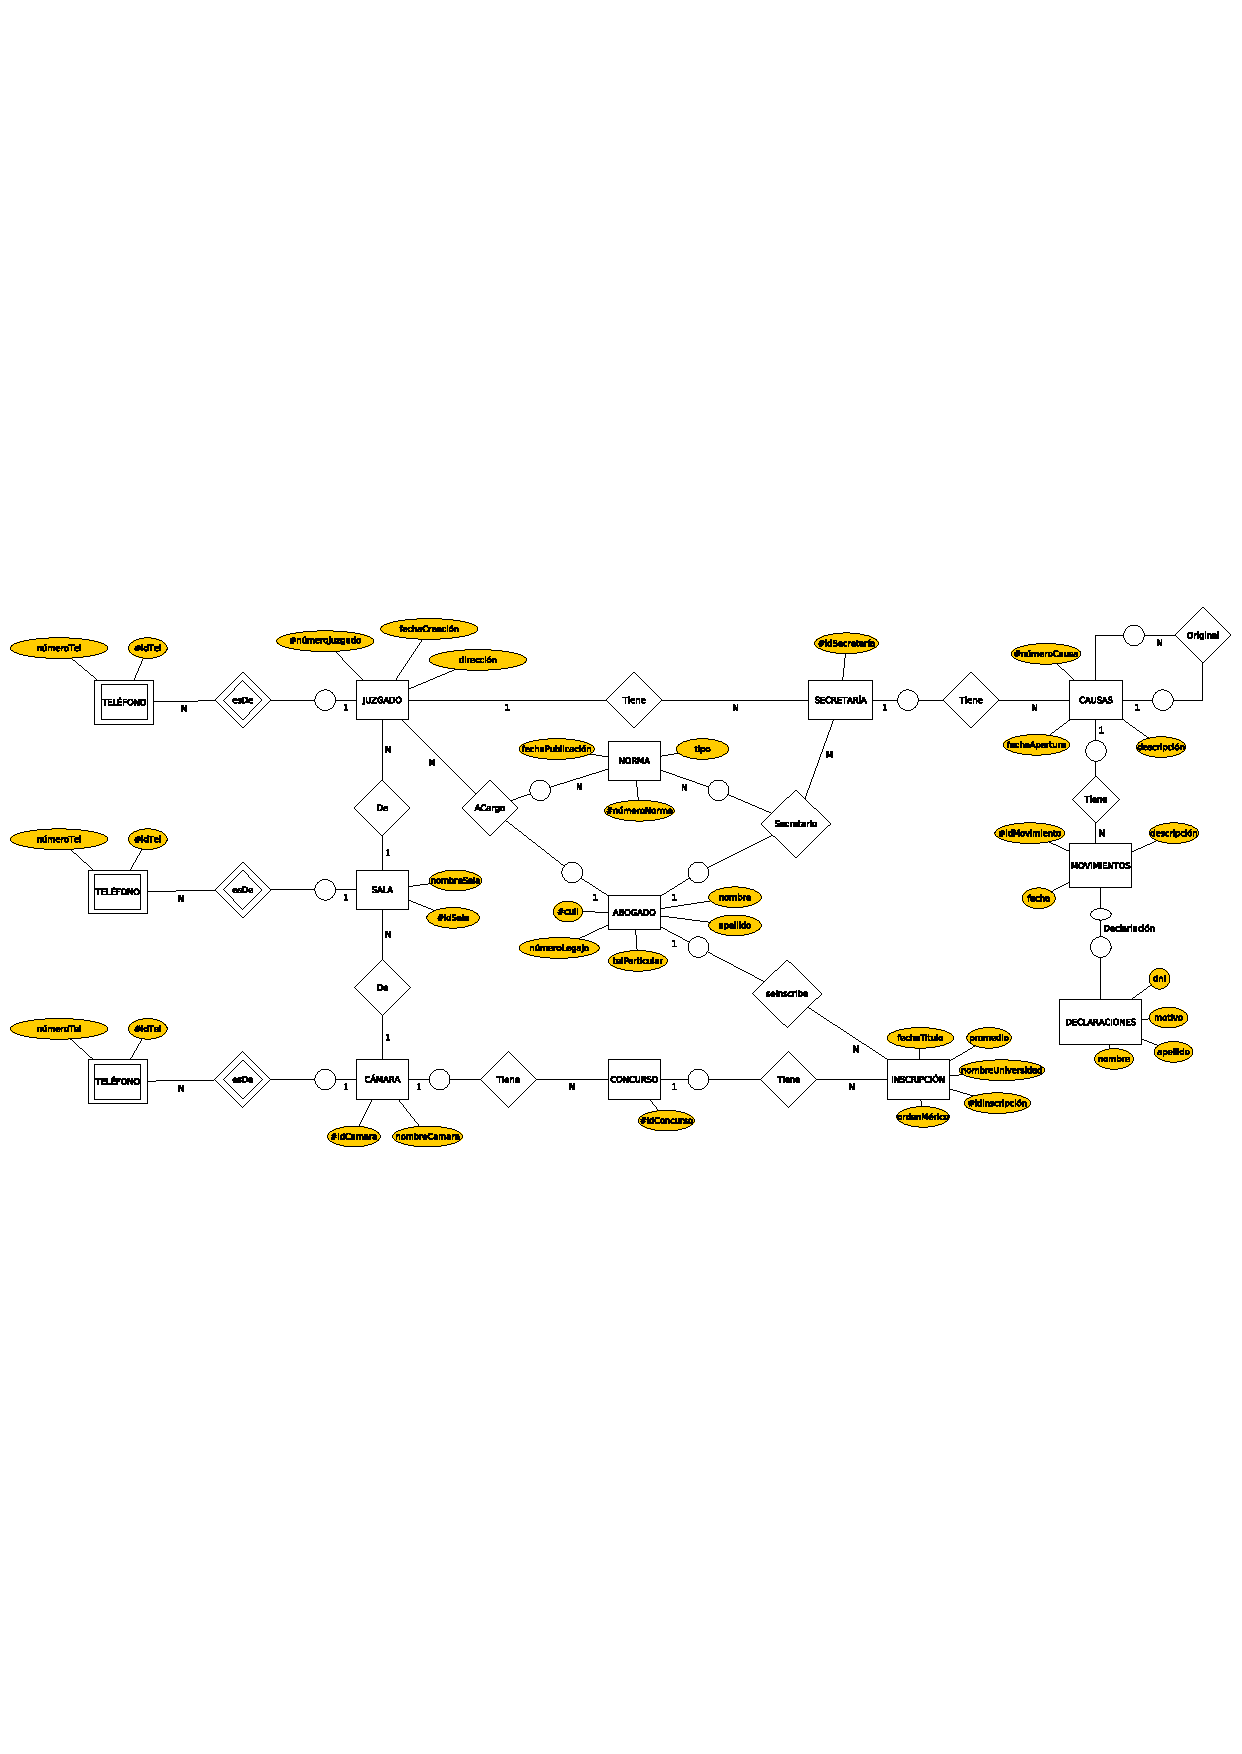
\includegraphics[width=0.8\textwidth]{DER.pdf}}}
% \scalebox{1.0}{\rotatebox{-90}{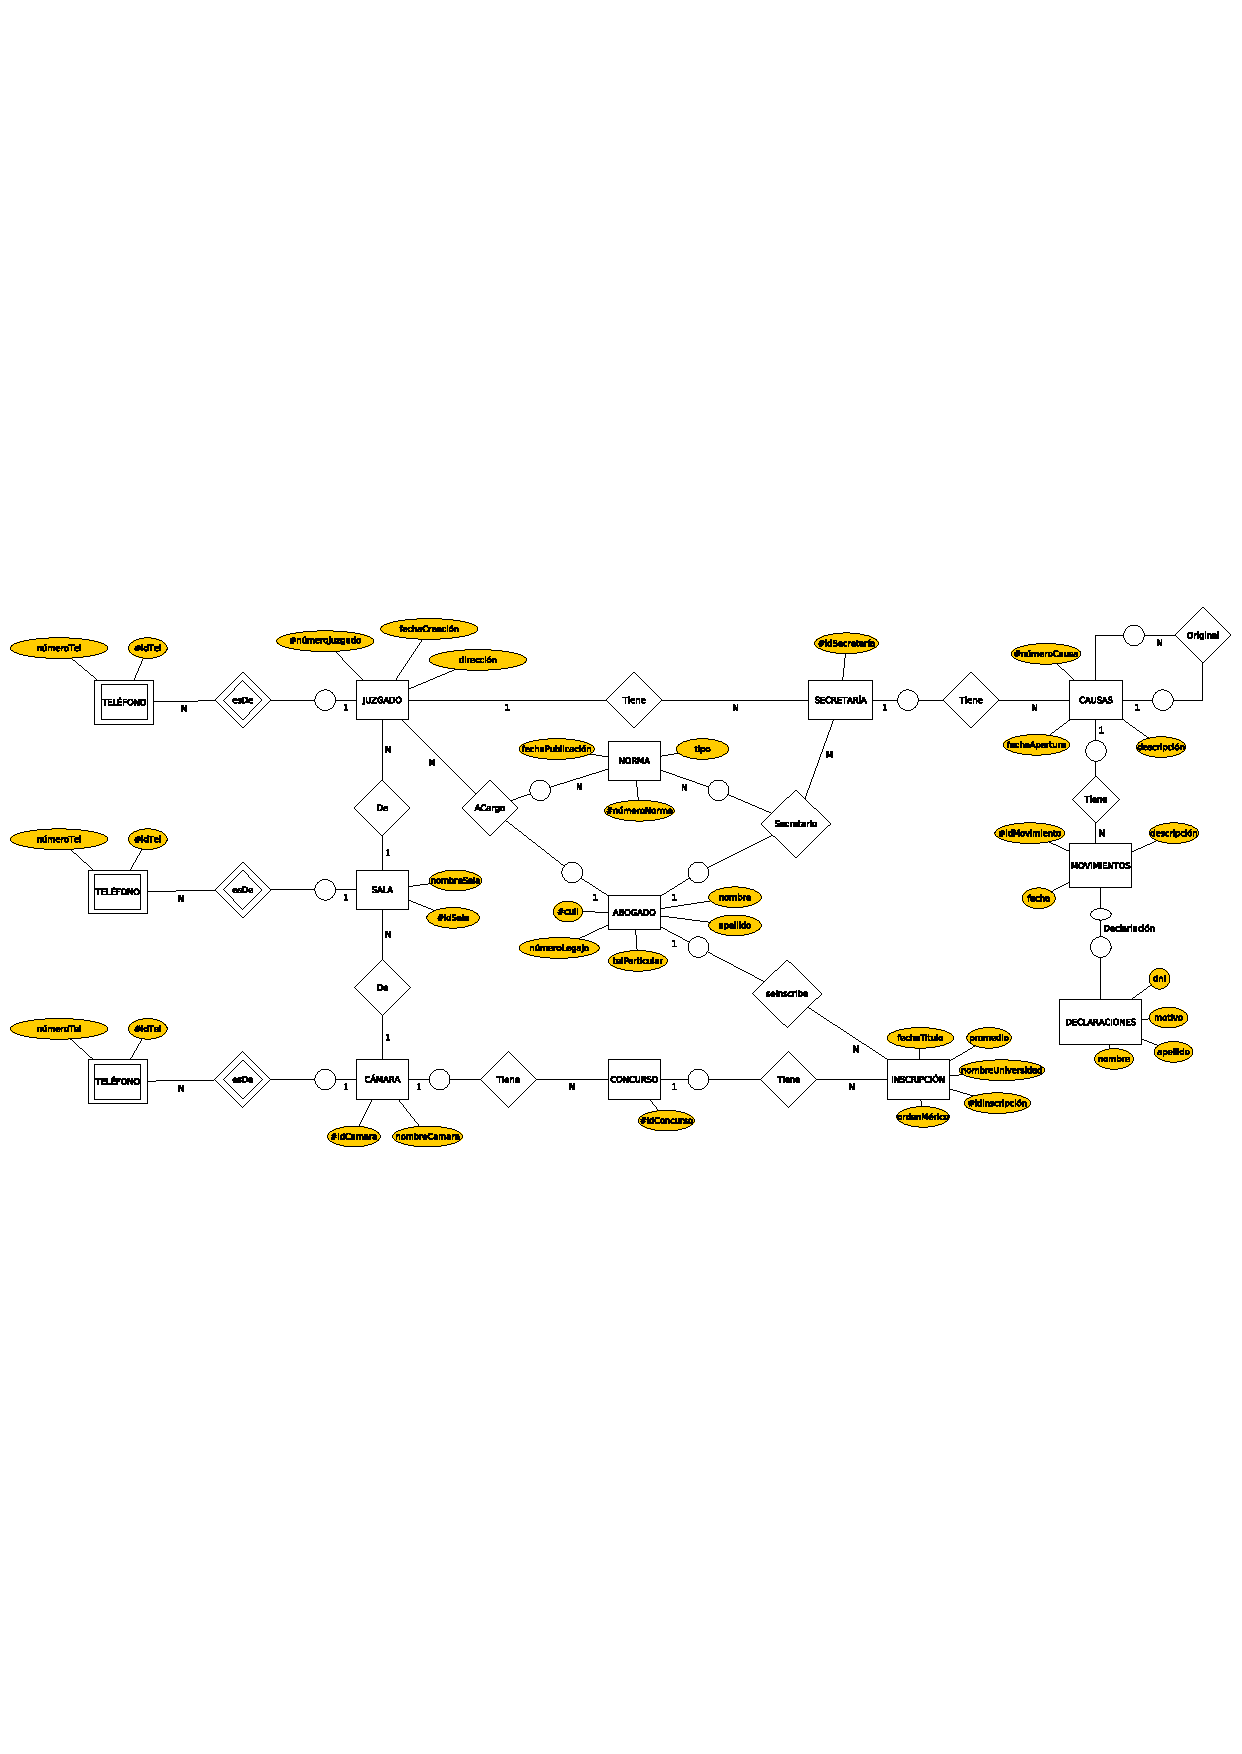
\includegraphics[width=1.0\textwidth]{DER.pdf}}}
\caption{DER}
\end{figure}

\newpage
Restricciones adicionales al DER:

\begin{itemize}
\item Toda causa esta en un y solo un rol de la interrelación unaria. Es decir, o es la original para un tema dado, o es copia de otra anterior.
\item Un Abogado no puede tener dos inscripciones diferentes para el mismo concurso. Esta restricción se podría evitar con un modelado diferente, pero en las explicaciones subsecuentes se verá porque se optó por este modelo.
\item Una norma debe designar al menos un juez o un secretario.
\end{itemize}



A continuación, se detallará cuales fueron las decisiones importantes a la hora de realizar el Diagrama de Entidad Relación:


En primer lugar, el grupo se encontró con diferentes opciones para modelar las normas que rigen los nombramientos de los jueces y los secretarios. 
Se explicará solamente el caso de las interrelacion entre Abogado, Norma y Juzgado, dado que la relación entre Abogado, Norma y Secretaría es análoga.

Las dos opciones principales consistían en una interrelación ternaria por un lado, y una agregación por el otro.
En el caso de la agregación, la idea se basaba en relacionar Abogado con Juzgado y, al hacer una agregación entre estos dos, interrelacionarlos con las normas. Sin embargo, este modelo traía aparejado una interpretación distinta a la requerida por el enunciado. En caso de utilizar esta forma, se hubiese permitido tener una norma relacionada dos veces con el mismo abogado, pero con diferente juzgado, lo cual no es valido. 

Dado lo explicado anteriormente, se optó por utilizar una relación ternaria, dado que se ajustaba mejor a los requerimientos elicitados. 
Es importante destacar que era necesario una relación de este tipo para lograr \textit{tener historia} en las normas; ya que dado que una norma tiene fecha de publicación, podría ser que dos normas diferentes hagan referencia al mismo par de Juzgado y Abogado.


\bigskip

En segundo lugar, se mostrará porque las inscripciones se encuentra modeladas de la forma presentada. 

Al tener las inscripciones como una entidad relacionada con los Abogados y con los Concursos, necesitamos la restricción adicional que dice que un Abogado no puede tener dos Inscripciones para el mismo Concurso. Existe otra forma de modelar esto que sería unir directamente Abogado con Concursos, y poner todos los atributos respectivos a la Inscripción en la interrelación. Si bien esto es valido y hubiese evitado la restricción adicional, se consideró que la inscripción tenia fuerza y una cantidad de atributos necesaria como para ser considerada una entidad aparte.

\bigskip

En último lugar, se explicará la interrelación unaria en las causas. 

Dado que las causas se deben agrupar por los hechos a los que hacen referencia, se barajó la idea de poner el motivo de la causa como una entidad aparte, pero se consideró que esto no tenía una relevancia necesaria como para ser modelado con una entidad nueva. 

De esta manera, se optó una interralación unaria que relaciona las causas entre sí dependiendo del motivo de las mismas. Para realizar esto, se vieron diferentes maneras de hacerlo. Las diferentes maneras estaban basadas en la cardinalidad y la participación de las causas. Finalmente, se eligió utilizar una interrelación con cardinalidad 1:N, en donde la interpretación de la misma es que para un motivo dado hay una causa original que fue la primera en llegar, y luego estan las causas del mismo hecho que llegaron despues que tiene una foreign key a la causa original.

\newpage

\newpage

\section{Modelo Relacional Derivado}

Aca quedan pendientes del MR.\\

TODO: Chequear si la foreing key en las debiles va subrayada o no (dado q en el manual no esta subrayada)
TODO: Hacer Restricciones de la relacion unaria \\
TODO: No se como poner la referencia de CAUSAS me marece lo de la interrelacion unaria.
\begin{itemize}

\item TELÉFONO\_J( \underline{idTel}, \underline{númeroJuzgado}, númeroTel) 
	\begin{itemize}
		\item CK = \{(idTel, númeroJuzgado)\}
		\item PK = \{(idTel, númeroJuzgado)\}
		\item FK = \{(númeroJuzgado)\}
		\item númeroJuzgado hace referencia a JUZGADO.númeroJuzgado.
		\item Restricciones:
			\begin{itemize}
			\item  TELÉFONO\_J.númeroJuzgado debe estar en JUZGADO.númeroJuzgado.
			\\
			
			\end{itemize}
	\end{itemize}	

	
\item JUZGADO( \underline{númeroJuzgado}, fechaCreación, dirección, \dashuline{idSala})
	\begin{itemize}
		\item CK = \{(númeroJuzgado)\}
		\item PK = \{(númeroJuzgado)\}
		\item FK = \{(idSala)\}
		\item Restricciones:
		\item idSala hace referencia a SALA.idSala.
			\begin{itemize}
			\item JUZGADO.númeroJuzgado puede no estar en TELÉFONO\_J.númeroJuzgado.
			\item JUZGADO.idSala no puede ser NULO.
			\item JUZGADO.númeroJuzgado debe estar en ACARGO.númeroJuzgado.
			\\
			\end{itemize}
	\end{itemize}


\item TELÉFONO\_S( \underline{idTel}, \underline{idSala}, númeroTel) 
	\begin{itemize}
		\item CK = \{(idTel, idSala)\}
		\item PK = \{(idTel, idSala)\}
		\item FK = \{(idSala)\}
		\item idSala hace referncia a SALA.idSala.
		\item Restricciones:
			\begin{itemize}
			\item TELÉFONO\_S.idSala debe estar en  SALA.idSala.
			\\
			\end{itemize}
	\end{itemize}


\item SALA( \underline{idSala}, nombreSala, \dashuline{idCámara},dirección)
	\begin{itemize}
		\item CK = \{(idSala)\}
		\item PK = \{(idSala)\}
		\item FK = \{(idCámara)\}
		\item idCámara hace referencia a CÁMARA.idCámara.
		\item Restricciones:
			\begin{itemize}
			\item SALA.idSala puede no estar en TELÉFONO\_S.idSala.
			\item SALA.idCámara no puede ser NULO.
			\\
			\end{itemize}
	\end{itemize}
	
	
\item TELÉFONO\_C( \underline{idTel}, \underline{idCámara}, númeroTel) 
	\begin{itemize}
		\item CK = \{(idTel, idCámara)\}
		\item PK = \{(idTel, idCámara)\}
		\item FK = \{(idCámara)\}
		\item idCámara hace referencia referencia a CÁMARA.idCámara.
		\item Restricciones:
			\begin{itemize}
			\item TELÉFONO\_C.idCámara debe estar en CÁMARA.idCámara.
			\\
			\end{itemize}
	\end{itemize}


\item CÁMARA( \underline{idCámara}, nombreCámara, dirección)
	\begin{itemize}
		\item CK = \{(idCámara)\}
		\item PK = \{(idCámara)\}
		\item FK = \{ \}
		\item Restricciones:
			\begin{itemize}
			\item CÁMARA.idCámara debe estar en TELÉFONO\_C.idTeléfono.
			\item CÁMARA.idCámara puede no estar en CONCURSO.idCámara.
			\\			
			\end{itemize}
	\end{itemize}
		
	
\item CONCURSO( \underline{idConcurso},fecha,\dashuline{idCámara})
	\begin{itemize}
		\item CK = \{(idConcurso)\}
		\item PK = \{(idConcurso)\}
		\item FK = \{(idCámara)\}
		\item idCámara hace referencia a CÁMARA.idCámara.
		\item Restricciones:
			\begin{itemize}
			\item CONCURSO.idCámara no puede ser NULO.
			\item CONCURSO.idConcurso puede no estar en INSCRIPCIÓN.idConcurso.
			\\			
			\end{itemize}		
	\end{itemize}
	
	
\item INSCRIPCIÓN( \underline{idInscripción}, ordenMérito, nombreUniversidad, promedio, fechaTitulo, \dashuline{idConcurso}, \dashuline{cuil})
	\begin{itemize}
		\item CK = \{(idInscripción)\}
		\item PK = \{(idInscripción)\}
		\item FK = \{(idConcurso),(cuil)\}
		\item idConcurso hace referencia a CONCURSO.idConcurso.
		\item cuil hace referencia a ABOGADO.cuil.
		\item Restricciones:
			\begin{itemize}
			\item INSCRIPCIÓN.idConcurso no puede ser NULO.
			\item INSCRIPCIÓN.cuil no puede ser NULO.
			\\
			\end{itemize}
	\end{itemize}
	
	
\item ABOGADO( \underline{cuil}, númerodeLegajo, telParticular, apellido, nombre)
	\begin{itemize}
		\item CK = \{(cuil)\}
		\item PK = \{(cuil)\}
		\item FK = \{\}
		\item Restricciones:
			\begin{itemize}
			\item ABOGADO.cuil puede no estar en INSCRIPCIÓN.cuil.
			\item ABOGADO.cuil puede no estar en ACARGO.cuil.
			\item ABOGADO.cuil puede no estar en SECRETARIO.cuil.
			\\
			\end{itemize}
	\end{itemize}

	
\item NORMA( \underline{númeroNorma}, fechaPublicación, tipo)
	\begin{itemize}
		\item CK = \{(númeroNorma)\}
		\item PK = \{(númeroNorma)\}
		\item FK = \{\}
		\item Restricciones:
			\begin{itemize}
			\item NORMA.númeroNorma puede no estar en ACARGO.númeroNorma.
			\item NORMA.númeroNorma puede no estar en SECRETARIO.númeroNorma.
			\\
			\end{itemize}
	\end{itemize}

	
\item ACARGO(  \underline{númeroNorma}, \underline{númeroJuzgado}, \dashuline{cuil})
	\begin{itemize}
		\item CK = \{(númeroNorma,númeroJuzgado)\}
		\item PK = \{(númeroNorma,númeroJuzgado)\}
		\item FK = \{(cuil)\}
		\item cuil hace referencia a ABOGADO.cuil.
		\item Restricciones:
			\begin{itemize}
			\item ACARGO.númeroJuzgado debe estar en JUZGADO.númeroJuzgado.
			\item ACARGO.númeroNorma debe estar en NORMA.númeroNorma.
			\item ACARGO.cuil debe estar en ABOGADO.cuil.
			\\
			\end{itemize}
	\end{itemize}
	
	
\item SECRETARIO( \underline{númeroNorma}, \underline{idSecretaría}, \dashuline{cuil})
	\begin{itemize}
		\item CK = \{(númeroNorma,idSecretaría)\}
		\item PK = \{(númeroNorma,idSecretaría)\}
		\item FK = \{(cuil)\}
		\item cuil hace referencia a ABOGADO.cuil.
		\item Restricciones:
			\begin{itemize}
			\item SECRETARIO.númeroNorma debe estar en NORMA.númeroNorma.
			\item SECRETARIO.cuil debe estar en ABOGADO.cuil.
			\item SECRETARIO.idSecretaría debe estar en SECRETARÍA.
			\\
			\end{itemize}
	\end{itemize}


\item SECRETARÍA( \underline{idSecretaría}, \dashuline{númeroJuzgado})
	\begin{itemize}
		\item CK = \{(idSecretaría)\}
		\item PK = \{(idSecretaría)\}
		\item FK = \{(númeroJuzgado)\}
		\item númeroJuzgado hace referencia JUZGADO.númeroJuazgado.
		\item Restricciones:
			\begin{itemize}
			\item SECRETARÍA.númeroJuzgado no puede ser NULO.
			\item SECRETARÍA.idSecretaría puede no estar en CAUSAS.idSecretaría.
			\item SECRETARÍA.idSecretaría debe estar en SECRETARIO.idSecretaria.
			\\
			\end{itemize}
	\end{itemize}

	
\item CAUSAS( \underline{númeroCausa}, fechaApertura, descripción, \dashuline{númeroCausaOriginal}, \dashuline{idSecretaría})
	\begin{itemize}
		\item CK = \{(númeroCausa)\}
		\item PK = \{(númeroCausa)\}
		\item FK = \{(númeroCausaOriginal),(idSecretaría)\}
		\item 
		\item Restricciones:
			\begin{itemize}
			\item CAUSAS.idSecretaría no puede ser NULO.
			\item CAUSAS.númeroCausa puede no estar en MOVIMIENTOS.númeroCausa.
			\\
			\end{itemize}
			TODO: Las Restricciones de las unarias requieren definir roles creo, lo cuelgo.
	\end{itemize}

	
\item MOVIMIENTO( \underline{idMovimiento}, descripción, fecha, \dashuline{númeroCausa}, tipo)
	\begin{itemize}
		\item CK = \{(idMovimiento)\}
		\item PK = \{(idMovimiento)\}
		\item FK = \{(númeroCausa)\}
		\item númeroCausa hace referencia a CAUSA.númeroCausa.
		\item Restricciones:
			\begin{itemize}
			\item MOVIMIENTO.idMovimiento puede no estar en DECLARACIONES.idMovimiento.
			\\
			\end{itemize}
	\end{itemize} 
	
\item DECLARACIONES(\underline{idMovimiento}, dni, motivo, apellido, nombre)
	\begin{itemize}
		\item CK = \{ \}
		\item PK = \{ \}
		\item FK = \{ \}
		\item Restricciones:
			\begin{itemize}
			\item DECLARACIONES.idMovimiento debe estar en MOVIMIENTO.idMovimiento.
			\\
			\end{itemize}
	\end{itemize}
	
	
\end{itemize}		

\newpage


\section{Store Procedures/Triggers}

Para realizar las consultas que fueron requeridas por las consignas del trabajo se decidió implementar las soluciones mediante Stored Procedures, para de esta forma poder acceder a las mismas de forma sencilla y cómoda.

\underline{Consulta:}

\textbf{El nombre de las salas que más declaraciones tomaron en el último año.}

Esta consulta es generada mediante el siguiente código:

\begin{verbatim}

SELECT nombre 'Nombre de la Sala', declaraciones 'Cantidad de Declaraciones'
FROM sala, (
	SELECT id_sala, count( * ) declaraciones
	FROM juzgado, (
		SELECT id_juzgado
		FROM secretaria, (
			SELECT id_secretaria
			FROM causas, (
				SELECT *
				FROM movimiento
				WHERE id
				IN (
					SELECT id_movimiento
					FROM declaraciones
				)
				) AS movConDec
			WHERE movConDec.id_causa = causas.id
			)secConDec
		WHERE secConDec.id_secretaria = secretaria.id
		) AS juzConDec
	WHERE juzConDec.id_juzgado = juzgado.id
	GROUP BY id_sala
	) AS salaConDec
WHERE sala.id = salaConDec.id_sala
ORDER BY declaraciones DESC
LIMIT 0 , 30

\end{verbatim}

La idea que se implemento es ir recorriendo desde las movimientos que fueron declaraciones hasta llegar a las Salas donde estos fueron originados, para ello se fue asociando las identificaciones correspondientes que enlazaban las diferentes tablas durante el camino. De esta forma se obtuvo una tabla con un campo sala y otro que indica la cantidad de declaraciones que fueron tomadas por la misma. Luego se procedió a ordenarlas de forma decreciente según la cantidad de declaraciones.

Se denomino \textbf{ranking()}, al Stored Procedure que implementa esta consulta.

\bigskip


\underline{Consulta:}

\textbf{El nombre de los jueces/secretarios que fueron nombrados por cada cámara a pesar de haber postulantes con un orden de mérito mejor que aún no habían sido designados.}

Esta consulta es generada mediante el siguiente código:

\begin{verbatim}
SELECT DISTINCT nombre
FROM    abogado AS a, concurso AS c, acargo, 
        inscripcion AS i, norma AS n, secretario AS s
WHERE   
    (a.cuil = acargo.cuil_abogado OR a.cuil = s.cuil_abogado) 
    -- El abogado a fue nombrado juez o secretario

    AND a.cuil = i.cuil_abogado 
    -- La inscripcion i corresponde al abogado a

    AND c.id = i.id_concurso  
    -- La inscripcion i corresponde al concurso c

    AND c.id IN 
    -- El concurso c es el que esta vigente para la norma n.
    -- Es decir, c es el ultimo concurso antes de que se publicara la norma n.
    (
    SELECT id
    FROM concurso AS conc
    WHERE   
        conc.fecha <= n.fecha_publicacion
        AND (conc.fecha >= ALL (
            SELECT fecha
            FROM concurso conc1
            WHERE conc1.fecha <= n.fecha_publicacion
            ))
    )
    AND EXISTS (    
    -- Existe un abogado inscripto en el mismo concurso,  
    -- con menor orden de merito, que
    -- no esta entre los nombrados jueces o secretarios.
    SELECT *
    FROM abogado AS abog, inscripcion AS insc
    WHERE   
        abog.cuil = insc.cuil_abogado 
        -- La inscripcion insc corresponde al abogado abog.
        AND insc.orden_merito < i.orden_merito  
        -- El orden de merito de la inscripcion insc
        -- es menor que el de la inscripcion i.
        AND insc.id_concurso = i.id_concurso    
        -- Las inscripciones insc e i 
        -- corresponden al mismo concurso
        AND NOT EXISTS (    
        -- No esta nombrado el abogado abog por una norma que 
        -- corresponda al concurso c.
            SELECT *
            FROM norma AS norm, acargo AS acargo2, secretario AS secretario2
            WHERE  
               norm.fecha_publicacion <= n.fecha_publicacion 
               -- La norma norm es anterior a la norma n
               AND norm.fecha_publicacion >= c.fecha    
               -- El concurso c ya estaba vigente cuando 
               -- se hizo la norma norm.
               AND 
               -- El abogado aparece nombrado juez o aparece nombrado 
               -- secretario bajo la norma norm.
                   (
                       (acargo2.cuil_abogado = abog.cuil 
                       -- El abogado abog aparece nombrado juez.
                       AND norm.id = acargo2.id_norma 
                       -- El nombramiento corresponde a la norma norm.
                       ) 
                    OR 
                       (secretario2.cuil_abogado = abog.cuil 
                       -- El abogado abog aparece nombrado secretario.
                       AND norm.id = secretario2.id_norma 
                       -- El nombramiento corresponde a la norma norm.
                       ) 
                   )
            )
    )
\end{verbatim}

Para resolver la consulta se identifican un abogado, la norma que lo nombra como juez o secretario y a su inscripción en el concurso vigente al momento de publicarse esa norma. Logrado esto, se buscan los abogados que tenían mejor posición en el orden de mérito del concurso vigente para los cuales no existía ninguna norma que los nombrara. Si este último conjunto no es vacío, entonces el abogado identificado fue nombrado habiendo todavía postulantes con un orden de mérito mejor que aún no habían sido designados.
Se denominó \textbf{acomodados()} al Stored Procedure con la intención de reflejar con un poco de humor la principal característica de los abogados cuyos nombres aparecen.

\bigskip


\underline{Control:}

\textbf{Registro automático de datos de control de las altas, bajas y modificaciones de concursos y sus resultados}

Para realizar esta tarea usamos la funcionalidad que nos provee el motor de la base de datos llamada "disparadores" o "triggers". La idea es llevar el control de los cambios que se realizan en las tablas relacionadas con la gestión de los concursos (Concurso e Inscripción). Para realizar esto creamos un conjunto de disparadores que registran los movimientos que se realizan en estas tablas y guardan dicha información en otras tablas creadas únicamente para este propósito.

El siguiente código implementa los triggers que mencionamos anteriormente:

\begin{verbatim}
CREATE TRIGGER auditoria_concurso_ins AFTER INSERT ON concurso
FOR EACH ROW
INSERT INTO auditoria_concurso(tipo, new_id_camara, new_id_concurso
,new_fecha, usuario, fecha)
VALUES ('Ins',NEW.id_camara, NEW.id,NEW.fecha, CURRENT_USER(), NOW());

CREATE TRIGGER auditoria_concurso_del AFTER DELETE ON concurso
FOR EACH ROW
INSERT INTO auditoria_concurso(tipo, old_id_camara, old_id_concurso,
old_fecha,usuario, fecha)
VALUES ('Del',OLD.id_camara, OLD.id,OLD.fecha, CURRENT_USER(), NOW());

CREATE TRIGGER auditoria_concurso_upd AFTER UPDATE ON concurso
FOR EACH ROW
INSERT INTO auditoria_concurso(tipo, new_id_camara, new_id_concurso,
old_id_camara,old_id_concurso, old_fecha,new_fecha,usuario, fecha)
VALUES ('Upd',NEW.id_camara, NEW.id,OLD.id_camara, OLD.id,OLD.fecha, 
NEW.fecha, CURRENT_USER(), NOW());

CREATE TRIGGER auditoria_inscripcion_ins AFTER INSERT ON inscripcion
FOR EACH ROW
INSERT INTO auditoria_inscripcion(tipo, new_id, new_orden_merito, 
new_nombre_universidad, new_promedio, new_fecha_titulo, new_id_concurso,
 new_cuil_abogado, usuario, fecha)
VALUES ('Ins',NEW.id, NEW.orden_merito, NEW.nombre_universidad,
 NEW.promedio, NEW.fecha_titulo, NEW.id_concurso, NEW.cuil_abogado,
  CURRENT_USER() , NOW());

CREATE TRIGGER auditoria_inscripcion_del AFTER DELETE ON inscripcion
FOR EACH ROW
INSERT INTO auditoria_inscripcion(tipo, old_id, old_orden_merito, 
old_nombre_universidad, old_promedio, old_fecha_titulo, old_id_concurso,
 old_cuil_abogado, usuario, fecha)
VALUES ('Del',OLD.id, OLD.orden_merito, OLD.nombre_universidad, 
OLD.promedio, OLD.fecha_titulo, OLD.id_concurso, OLD.cuil_abogado, 
CURRENT_USER() , NOW());

CREATE TRIGGER auditoria_inscripcion_upd AFTER UPDATE ON inscripcion
FOR EACH ROW
INSERT INTO auditoria_inscripcion(tipo, old_id, old_orden_merito,
old_nombre_universidad, old_promedio, old_fecha_titulo, old_id_concurso,
old_cuil_abogado,new_id, new_orden_merito, new_nombre_universidad, new_promedio,
new_fecha_titulo, new_id_concurso, new_cuil_abogado, usuario, fecha)
VALUES ('Upd',OLD.id, OLD.orden_merito, OLD.nombre_universidad, OLD.promedio,
OLD.fecha_titulo, OLD.id_concurso, OLD.cuil_abogado,NEW.id, NEW.orden_merito,
NEW.nombre_universidad, NEW.promedio, NEW.fecha_titulo, NEW.id_concurso,
NEW.cuil_abogado, CURRENT_USER() , NOW());

\end{verbatim}



\newpage



\end{document}
